\let\negmedspace\undefined
\let\negthickspace\undefined
\documentclass[journal]{IEEEtran}
\usepackage[a5paper, margin=10mm, onecolumn]{geometry}
%\usepackage{lmodern} % Ensure lmodern is loaded for pdflatex
\usepackage{tfrupee} % Include tfrupee package

\setlength{\headheight}{1cm} % Set the height of the header box
\setlength{\headsep}{0mm}     % Set the distance between the header box and the top of the text

\usepackage{gvv-book}
\usepackage{gvv}
\usepackage{cite}
\usepackage{amsmath,amssymb,amsfonts,amsthm}
\usepackage{algorithmic}
\usepackage{graphicx}
\usepackage{textcomp}
\usepackage{xcolor}
\usepackage{txfonts}
\usepackage{listings}
\usepackage{enumitem}
\usepackage{mathtools}
\usepackage{gensymb}
\usepackage{comment}
\usepackage[breaklinks=true]{hyperref}
\usepackage{tkz-euclide} 
\usepackage{listings}
% \usepackage{gvv}                                        
\def\inputGnumericTable{}                                 
\usepackage[latin1]{inputenc}                                
\usepackage{color}                                            
\usepackage{array}                                            
\usepackage{longtable}                                       
\usepackage{calc}                                             
\usepackage{multirow}                                         
\usepackage{hhline}                                           
\usepackage{ifthen}                                           
\usepackage{lscape}
\begin{document}

\bibliographystyle{IEEEtran}
\vspace{3cm}

\title{1.1.5.13}
\author{EE24BTECH11047 - Niketh Prakash Achanta
}
% \maketitle
% \newpage
% \bigskip
{\let\newpage\relax\maketitle}

\renewcommand{\thefigure}{\theenumi}
\renewcommand{\thetable}{\theenumi}
\setlength{\intextsep}{10pt} % Space between text and floats

\numberwithin{figure}{enumi}
\renewcommand{\thetable}{\theenumi}


\textbf{Question}:\\
Find the ratio in which the $Y$ axis divides the line segment joining the points $\brak{5, -6}$
and $\brak{-1, -4}$. Also find the coordinates of the point of intersection. \hfill (10, 2012)
\\ \textbf{Solution: }\\
    \begin{table}[h!]    
      \centering
      \begin{center}
    \begin{tabular}{|c|c|c|} 
        \hline
            \textbf{Variable} & \textbf{Description} & \textbf{Formula} \\ 
        \hline
            $A$   & It is one end of the line segment & $A = \myvec{5 \\ -6}$ \\ 
        \hline
            $B$   & It is other end of line segment &  $B = \myvec{-1\\-4}$\\ 
        \hline
            $C$   & It is the point of intersection of line segment and $Y$-axis & $C  = \myvec{0\\y}$\\ 
        \hline
            $k$   & It is the ratio in which $C$ divides the line segment $AB$ & $C  = \brak{\frac{B + kA}{1 + k}}$\\ 
        \hline
    \end{tabular}
\end{center}  

      \caption{}
    \end{table}\\
Using the section formula:
    \begin{align}
        C  = \brak{\frac{B + kA}{1 + k}} \label{eq1.1.5.13.1}
    \end{align}
    \begin{align}
        C = \myvec{0 \\ y} \label{eq1.1.5.13.2}
    \end{align}
Also,
    \begin{align}
        C = \myvec{\frac{5k-1}{k+1} \\ \frac{-6k-4}{1+k}} \label{eq1.1.5.13.3}
    \end{align}
Solving for k using $x$ Coordinate of $C$
    \begin{align}
        \brak{\frac{5k-1}{k+1}} = 0  \label{eq1.1.5.13.4}
    \end{align}
    \begin{align}
        k = \frac{1}{5} = 0.2\label{eq1.1.5.13.5}
    \end{align}
Finding $y$ Coordinate of $C$ using $k$,
    \begin{align}
        y = \brak{\frac{-6k-4}{k+1}}  \label{eq1.1.5.13.6}
    \end{align}
    \begin{align}
        y = \brak{\frac{-1.2-4}{0.2+1}} \label{eq1.1.5.13.7}
    \end{align}
    \begin{align}
        y = -4.3334 \label{eq1.1.5.13.8}
    \end{align}
    \begin{figure}[h]
        \centering
       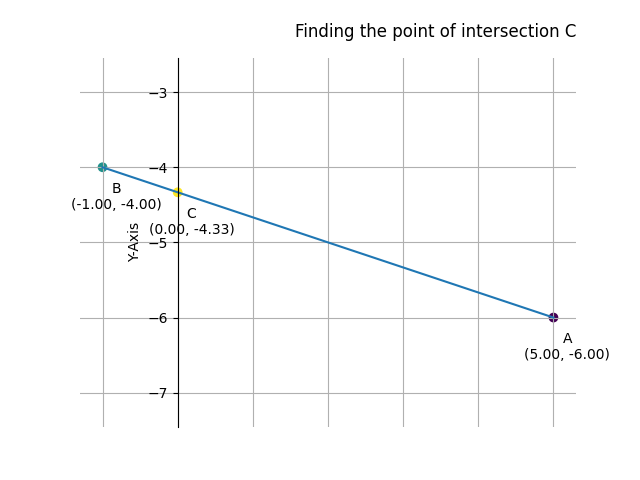
\includegraphics[width=0.7\linewidth]{figs/fig1.png}
       \caption{}
       \label{graph}
    \end{figure}
\end{document}  



